% Title     :: SamzaSQL: Scalable Fast Data Management with Streaming SQL
% Author    :: Milinda Pathirage
% Email     :: mpathira@indiana.edu
% Website   :: http://milinda.pathirage.org
% Template  :: sthlm beamer theme by Benjamin Weiss (hendryolson@gmail.com, http://v42.com), 
%              which is HEAVILY based on the HSRM beamer theme created by Benjamin Weiss
%			   (benjamin.weiss@student.hs-rm.de), which can be found on GitHub
%			   <https://github.com/hsrmbeamertheme/hsrmbeamertheme>.



%-=-=-=-=-=-=-=-=-=-=-=-=-=-=-=-=-=-=-=-=-=-=-=-=
%
%        LOADING DOCUMENT
%
%-=-=-=-=-=-=-=-=-=-=-=-=-=-=-=-=-=-=-=-=-=-=-=-=

\documentclass[newPxFont]{beamer}
\usetheme{sthlm}
%\usecolortheme{sthlmv42}

%-=-=-=-=-=-=-=-=-=-=-=-=-=-=-=-=-=-=-=-=-=-=-=-=
%        LOADING PACKAGES
%-=-=-=-=-=-=-=-=-=-=-=-=-=-=-=-=-=-=-=-=-=-=-=-=
\usepackage[utf8]{inputenc}
\usepackage{hyperref}
\usepackage{minted}
\usepackage{xcolor}
\usepackage{tikz}
\usepackage{tikz-qtree}
\usetikzlibrary{trees}
\usepackage{xxcolor}
\usetikzlibrary{shapes.misc,shapes.geometric,shapes.arrows,decorations.pathmorphing,decorations.shapes}
\usetikzlibrary{matrix,chains,scopes,positioning,arrows,fit}
\usepackage{smartdiagram}
\usesmartdiagramlibrary{additions}

\definecolor{computegreen}{RGB}{185, 224, 165}
\definecolor{datared}{RGB}{255, 204, 204}
\definecolor{dcpurple}{RGB}{229, 204, 255}


\usepackage{chronology}

\renewcommand{\event}[3][e]{%
  \pgfmathsetlength\xstop{(#2-\theyearstart)*\unit}%
  \ifx #1e%
    \draw[fill=black,draw=none,opacity=0.5]%
      (\xstop, 0) circle (.2\unit)%
      node[opacity=1,rotate=45,right=.2\unit] {#3};%
  \else%
    \pgfmathsetlength\xstart{(#1-\theyearstart)*\unit}%
    \draw[fill=black,draw=none,opacity=0.5,rounded corners=.1\unit]%
      (\xstart,-.1\unit) rectangle%
      node[opacity=1,rotate=45,right=.2\unit] {#3} (\xstop,.1\unit);%
  \fi}%

\newcommand{\specialcell}[2][l]{%
  \begin{tabular}[#1]{@{}l@{}}#2\end{tabular}}

%-=-=-=-=-=-=-=-=-=-=-=-=-=-=-=-=-=-=-=-=-=-=-=-=
%        BEAMER OPTIONS
%-=-=-=-=-=-=-=-=-=-=-=-=-=-=-=-=-=-=-=-=-=-=-=-=

%\setbeameroption{show notes}

%-=-=-=-=-=-=-=-=-=-=-=-=-=-=-=-=-=-=-=-=-=-=-=-=
%
%	PRESENTATION INFORMATION
%
%-=-=-=-=-=-=-=-=-=-=-=-=-=-=-=-=-=-=-=-=-=-=-=-=

\title{Horme}
\subtitle{Random Access Big Data Analytics}
%\date{\small{\jobname}}
%\date{\today}
\author{Guangchen Ruan, Beth Plale}
\institute{School of Informatics and Computing, Indiana University}

\hypersetup{
pdfauthor = {Milinda Pathirage: milinda.pathirage@gmail.com},
pdfsubject = {},
pdfkeywords = {},
pdfmoddate= {D:\pdfdate},
pdfcreator = {}
}

\begin{document}
\setbeamertemplate{caption}{\raggedright\insertcaption\par}

%-=-=-=-=-=-=-=-=-=-=-=-=-=-=-=-=-=-=-=-=-=-=-=-=
%
%	TITLE PAGE
%
%-=-=-=-=-=-=-=-=-=-=-=-=-=-=-=-=-=-=-=-=-=-=-=-=

\maketitle

%\begin{frame}[plain]
%	\titlepage
%\end{frame}

%-=-=-=-=-=-=-=-=-=-=-=-=-=-=-=-=-=-=-=-=-=-=-=-=
%
%	TABLE OF CONTENTS: OVERVIEW
%
%-=-=-=-=-=-=-=-=-=-=-=-=-=-=-=-=-=-=-=-=-=-=-=-=

\section{Introduction}

%-=-=-=-=-=-=-=-=-=-=-=-=-=-=-=-=-=-=-=-=-=-=-=-=
%	FRAME:
%-=-=-=-=-=-=-=-=-=-=-=-=-=-=-=-=-=-=-=-=-=-=-=-=
\begin{frame}[c]{Hathitrust Research Center (HTRC)}
Research arm of \textbf{Hathitrust Digital Library} that develops and maintain infrastructure for enabling computational access to \textbf{14 million} digitized volumes.

\vspace{1em}

\begin{exampleblock}{Mission}
Enable researchers world-wide to accomplish tera-scale text data-mining and analysis  
\end{exampleblock}
\end{frame}

\section{Motivation}

\begin{frame}[c]{HTRC Analytics Workflow}
\begin{figure}[ht!]
\smartdiagramset{back arrow disabled=true,
additions={
additional item offset=1em,
additional item height=0em,
additional item text width=15em,
additional arrow color=teal!40,
additional arrow line width=4pt,
additional connections disabled=false,
   additional arrow color=red,
   additional arrow tip=stealth,
   additional arrow line width=1pt
   }}
\smartdiagramadd[flow diagram:horizontal]{Selection,
  Retrieval, Analysis}{above of module2/{Data staging from Lustre/Data API},
  below of module1/{Select a subset of data for analysis (e.g. From 14 million volumes to 1 million)},
  below of module3/{MapReduce, Meandre, Custom Tools}}
\end{figure}
\end{frame}

\begin{frame}[c]{HTRC Analytics Infrastructure}


% Based on http://tex.stackexchange.com/questions/125234/upside-down-tikz-qtree-with-concentrated-edges

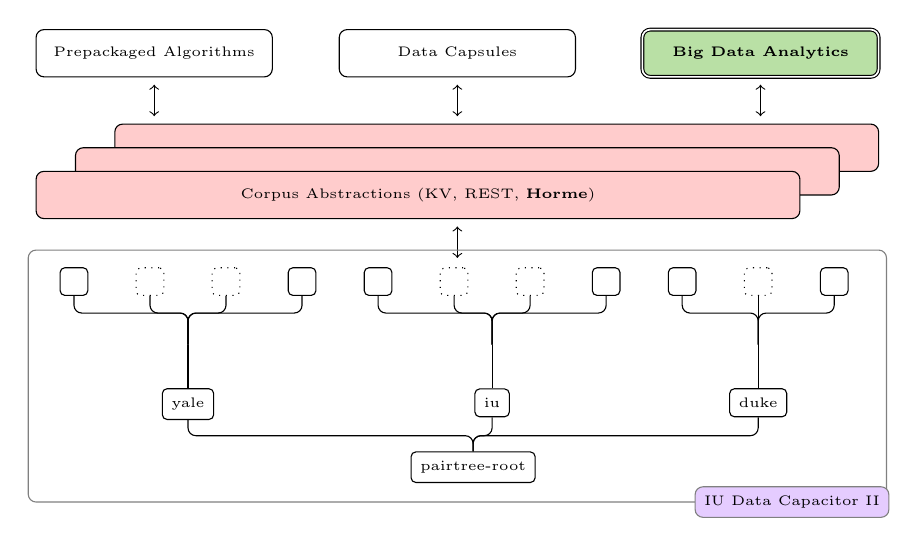
\begin{tikzpicture}
[   grow'=up,
    level distance=.8cm,
    sibling distance=.6cm,
    edge from parent fork up,
    edge from parent/.style={draw,rounded corners=1mm}
]
\begin{scope}[local bounding box=scope1]
  \draw[rounded corners=1mm] (-6.7,4.8) rectangle (-3.7,4.2) node[pos=.5] {\tiny Prepackaged Algorithms};
  \draw[rounded corners=1mm] (-2.85,4.8) rectangle (0.15,4.2) node[pos=0.5] {\tiny Data Capsules};
  \draw[rounded corners=1mm,fill=computegreen,double] (1,4.8) rectangle (4,4.2) node[pos=0.5] {\tiny \textbf{Big Data Analytics}};
  \draw[fill=datared,rounded corners=1mm] (-5.7,3.6) rectangle (4,3) ;
  \draw[fill=datared,rounded corners=1mm] (-6.2,3.3) rectangle (3.5,2.7) ;
  \draw[fill=datared,rounded corners=1mm] (-6.7,3) rectangle (3,2.4) node[pos=.5] {\tiny Corpus Abstractions (KV, REST, \textbf{Horme})};
\end{scope}
\draw[<->] (-1.35,2.3) -- (-1.35,1.9); %node[draw=orange,anchor=west,pos=0.5,circle,fill=red!20,inner sep=0pt,minimum size=10pt,xshift=2pt]{\footnotesize \textbf{1}};
\draw[<->] (-5.2,4.1) -- (-5.2,3.7); %node[draw=orange,anchor=west,pos=0.5,circle,fill=red!20,inner sep=0pt,minimum size=10pt,xshift=2pt]{\footnotesize \textbf{2}};
\draw[<->] (-1.35,4.1) -- (-1.35,3.7); %node[draw=orange,anchor=west,pos=0.5,circle,fill=red!20,inner sep=0pt,minimum size=10pt,xshift=2pt]{\footnotesize \textbf{3}};
\draw[<->] (2.5,4.1) -- (2.5,3.7); %node[draw=orange,anchor=west,pos=0.5,circle,fill=red!20,inner sep=0pt,minimum size=10pt,xshift=2pt]{\small \textbf{4}};
\begin{scope}[shift={($(scope1.north)+(0.2cm,-5.6cm)$)}]
  \tikzstyle{var} = [draw,shape=rectangle,minimum size=1em,rounded corners=0.6mm]
  \tikzstyle{operator} = [draw=none,fill=none,above,pos=0]
  \tikzset{every node/.style={var}}
  \Tree [.\tiny pairtree-root 
          [.\tiny yale [[.\node[] {}; ] [.\node[dotted] {}; ]  [.\node[dotted] {}; ] [.\node[] {}; ]]]
          [.\tiny iu [[.\node[] {}; ][.\node[dotted] {}; ] [.\node[dotted] {}; ][.\node[] {}; ]]]
          [.\tiny duke [[.\node[] {}; ] [.\node[dotted] {}; ] [.\node[] {}; ]] 
          ]
        ]
\end{scope}
\draw[rounded corners=1mm,draw,gray] (-6.8,2) rectangle (4.1,-1.2) node[fill=dcpurple,draw,pos=1,xshift=-1.2cm,rounded corners=1mm] {\tiny \textcolor{black}{IU Data Capacitor II}};
\end{tikzpicture}
\end{frame}

\begin{frame}[c]{Text Data Mining At HTRC}
  \begin{itemize}
    \item General pattern: 
    \begin{itemize}
      \item Reduce 14 million volumes to 1 million volumes
      \item Volumes are randomly distributed because volumes are organized based on the creator
      \item Access is by topics
    \end{itemize}
    \item HDFS performs poorly in random access use cases
    \item HBase is good for random access, but needs to deploy external to HPC or HTC compute nodes due to transient nature of batch jobs
    \item HBase over Lustre is not optimal
  \end{itemize}
\end{frame}


\begin{frame}[c]{Hadoop on HPC and HTC Environments}
\begin{columns}[T] % align columns
\begin{column}{.48\textwidth}
\begin{figure}[t]
  \includegraphics[scale=0.5]{hadoop-on-hpc}
  \centering
\end{figure}
\end{column}%
\hfill%
\begin{column}{.48\textwidth}
General workflow:
\begin{enumerate}
  \item Setup Hadoop cluster
  \item Stage input data
  \item Execute analysis algorithm
  \item Stage output data
\end{enumerate}
\end{column}%
\end{columns}

\end{frame}

\begin{frame}[c]{Hadoop on HPC and HTC Environments}
  \begin{itemize}
    \item Data is stored in a \emph{parallel file system} such as Lustre connected to compute nodes via network
    \item Often data get staged to the scratch space in compute nodes (e.g. HDFS data nodes) from Lustre before the actual computation
    \item Results get copied back to Lustre after job completion
    \item \textbf{High data staging overhead}
    \item HDFS on HPC and HTC environments is limited by scratch space capacity of compute nodes
  \end{itemize}
\end{frame}

\section{Horme}

\begin{frame}[c]{Horme}
\begin{itemize}
  \item Indexed binary file format for packing key/value pairs where size of the value range from couple of kilobytes to couple of megabytes
  \item A Set of tools for packing and managing key/value pairs  
  \item Library for reading and writing indexed binary files 
  \item Storage extensions for popular Big Data processing frameworks to read and write Horme binary files
  \item Not tied to any processing framework
  \item Works on top of any file system
  \item Delegates replication, file striping and fault-tolerance to underlying file system
\end{itemize}
\end{frame}

\begin{frame}[c]{Horme - BloomHashIndexFile}
\begin{figure}[t]
  \includegraphics[scale=0.6]{horme-2}
  \centering
\end{figure}  
\end{frame}

\begin{frame}[c]{Horme - Programming Abstraction}
  \begin{itemize}
    \item Reader
    \begin{center}
      \begin{tabular}{| l | l |}
       \hline
       \textbf{Scan} & \texttt{for(Record r : BloomHashIndexFile)} \\ 
       \hline
       \textbf{Random Access} & \texttt{Record get(Key key)} \\  
       \hline
       \textbf{Membership Test} & \texttt{boolean probablyHasKey(Key key)} \\    
       \hline
       \textbf{Accessors} & \specialcell{\texttt{HashIndex getHashIndex()} \\ 
\texttt{BloomFilter getBloomFilter()}} \\    
       \hline
      \end{tabular}
    \end{center}
    \item Writer
    \begin{center}
      \begin{tabular}{| l | l |}
       \hline
       \textbf{Write} & \texttt{void append(Key key, Value val)} \\ 
       \hline
       \textbf{Misc.} & \texttt{int getLength()} \\  
       \hline
      \end{tabular}
    \end{center}
  \end{itemize}
\end{frame}

\begin{frame}[c]{Horme - Distributed Packing Utility}
  \begin{itemize}
    \item Pack Key/Value style raw data to binary chunks
    \item Embarrassingly parallel packing process
    \item For the sake of load balancing each chunk should carry roughly the same payload
    \begin{itemize}
      \item Same \# of records (e.g., simulation analysis task)
      \item Same chunk file size (e.g., text mining task)
    \end{itemize}
  \end{itemize}
\end{frame}

\begin{frame}[c]{Horme - Parallel Processing Layer}
  \begin{itemize}
    \item Hadoop input and output format extension on top of BloomHashIndexFile
    \item Retains MapReduce Key/Value semantics 
    \item Support both scan and random access 
    \item Binary chunks can be served from a network file system or a HDFS cluster coupled with Hadoop deployment
  \end{itemize}
\end{frame}

\begin{frame}[c]{Horme - Processing from Network Storage}
\begin{figure}[t]
  \includegraphics[scale=0.4]{horme-with-pfs}
  \centering
\end{figure}
\end{frame}

\begin{frame}[c]{Horme - Processing from Network Storage}
\begin{itemize}
  \item With NLineInputFormat, a single input split consists of N consecutive lines
  \item \texttt{BloomHashIndexFile}'s \texttt{Reader} is used to read the value corresponding to each key in input split at mapper
  \item Input should be sorted by binary chunk's path so that the \texttt{RecordReader} only needs to opens a new file when the next line is a new chunk
  \item Workload is balanced with respect to number of records processed
  \item Workload is approximately balanced with respect to the size of the records 
\end{itemize}
\end{frame}

\begin{frame}[c]{Horme - Processing from HDFS}
  Horme's Hadoop extensions take care of figuring out input splits and converting input splits to key/value pairs for consumption by mappers.
  \begin{figure}[t]
  \includegraphics[scale=0.3]{horme-hdfs}
  \centering
\end{figure}
\end{frame}

\section{Evaluation}

\begin{frame}[c]{Environment}
\begin{itemize}
  \item For the single node setting, we conducted the experiment on a 4-core 2.4 GHz Intel W3503 Xeon CPU, 8 GB of memory, and 7200 RPM SATA drive. Each record has fixed sized key (100 byte) and value (2 MB).
  \item Hadoop v2.6.1
  \item HDFS uses 128 MB blocks with default replication factor of 3
  \item Karst compute nodes containing two Intel Xeon E5-2650 v2 8-core processors and 32 GB of RAM, and a local disk of 180 GB at 7200 rpm
  \item IU Datacapacitor II (Lustre) as parallel file system
\end{itemize}
\end{frame}

\begin{frame}[c]{Overhead of BloomHashIndexFile}
\vspace{-1.5cm}
\begin{columns}[T] % align columns
    \begin{column}{.48\textwidth}
    \begin{figure}[ht!]
      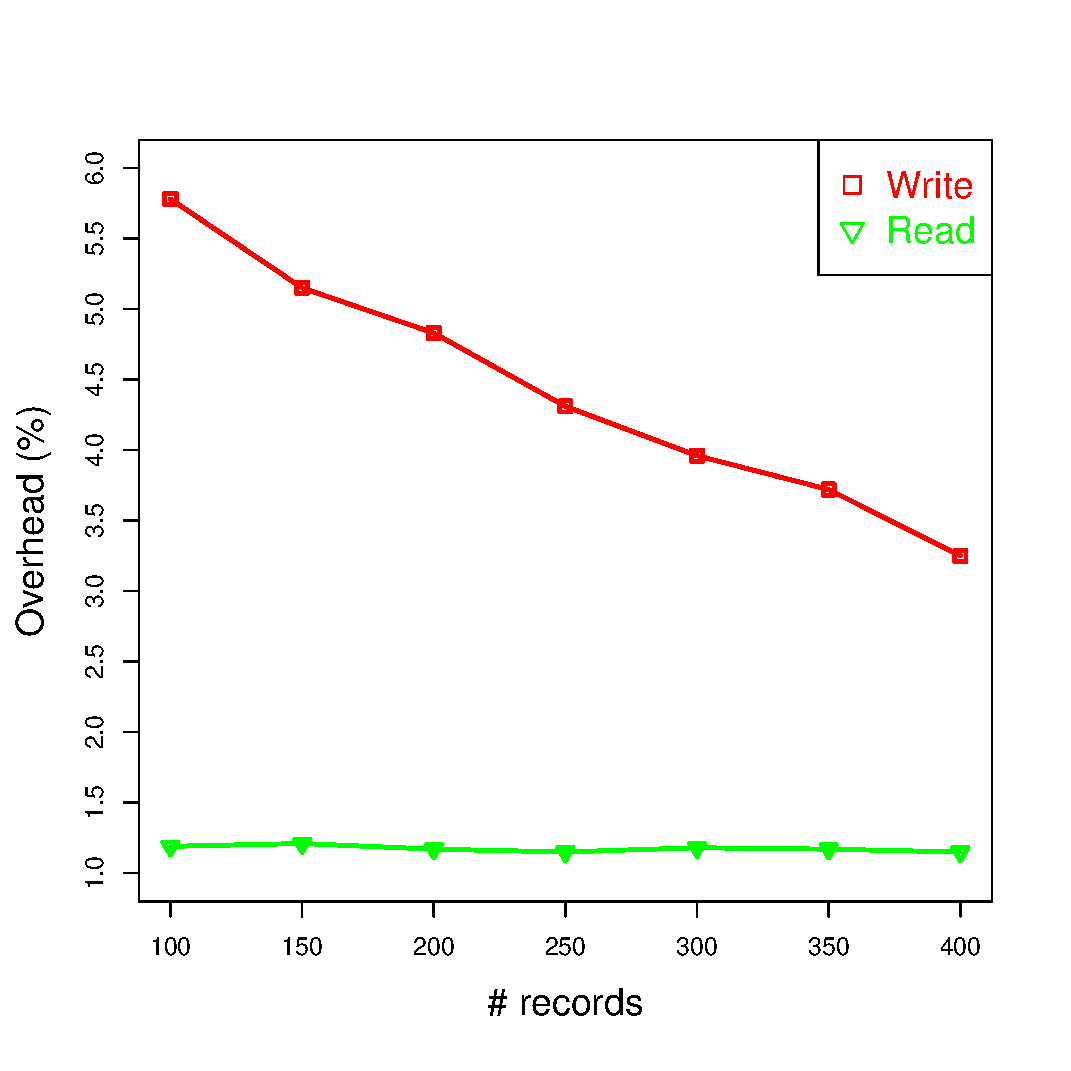
\includegraphics[scale=0.3]{exp-bloomhash-rw-overhead}
      \centering
    \end{figure}
    \end{column}%
    \hfill%
    \begin{column}{.48\textwidth}
    \begin{figure}[ht!]
      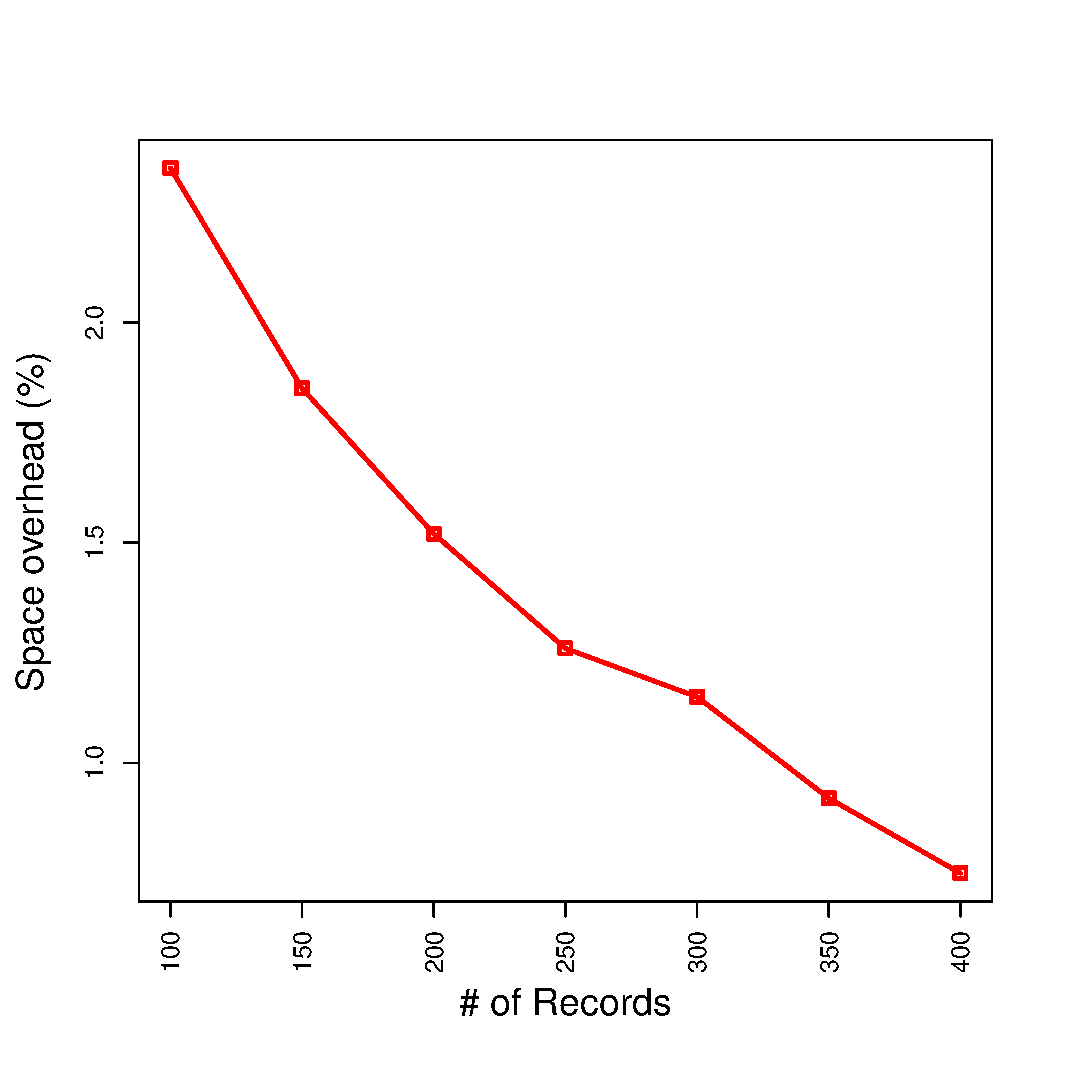
\includegraphics[scale=0.3]{exp-bloomhash-space-overhead}
      \centering
    \end{figure} 
    \end{column}%
\end{columns}  
\end{frame}

\begin{frame}[c]{Horme vs Vanilla Hadoop}
\vspace{-1.5cm}
\begin{columns}[T] % align columns
    \begin{column}{.48\textwidth}
    \begin{figure}[ht!]
      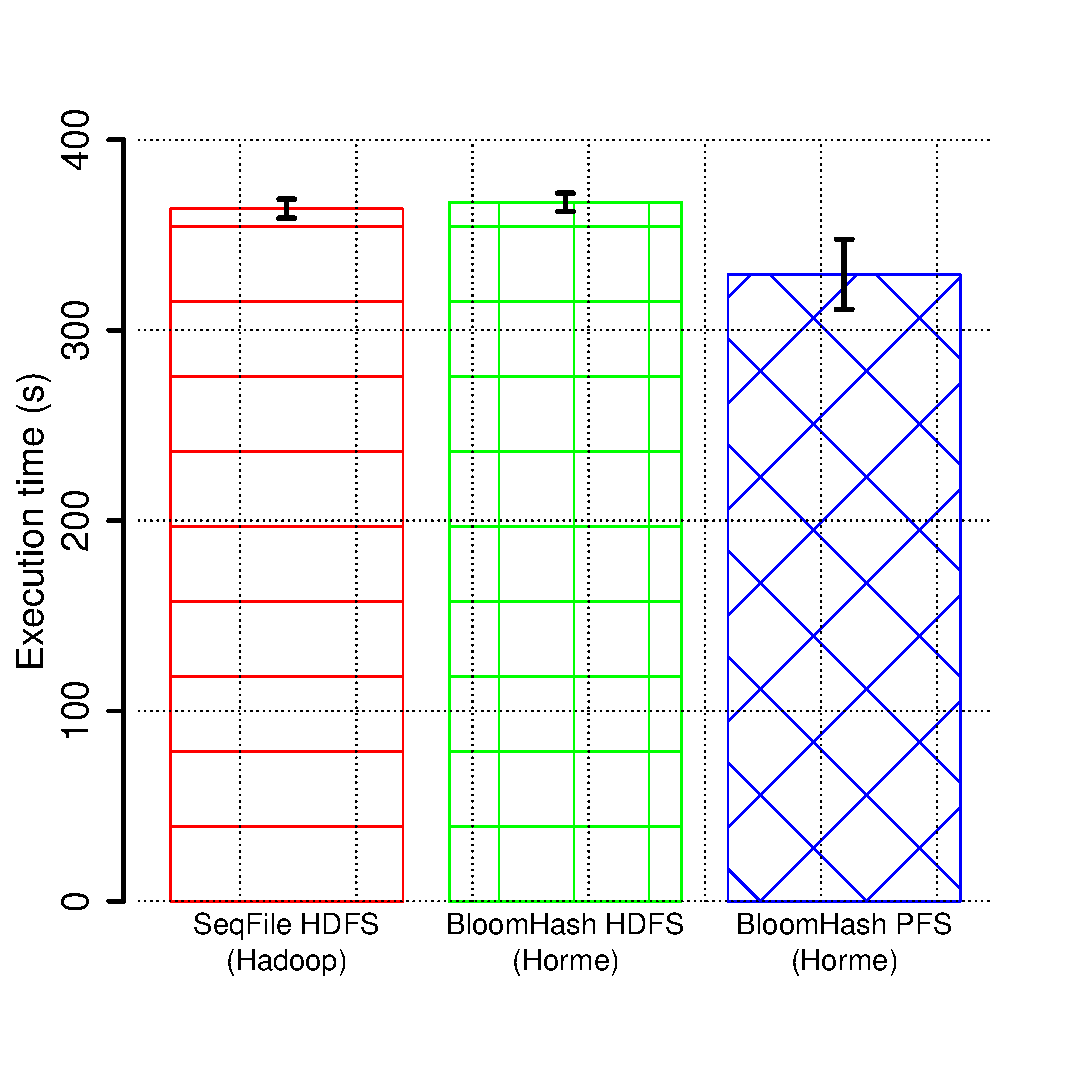
\includegraphics[scale=0.3]{eval-scan}
      \centering
      \caption{Scan/sequential Access}
    \end{figure}
    \end{column}%
    \hfill%
    \begin{column}{.48\textwidth}
    \begin{figure}[ht!]
      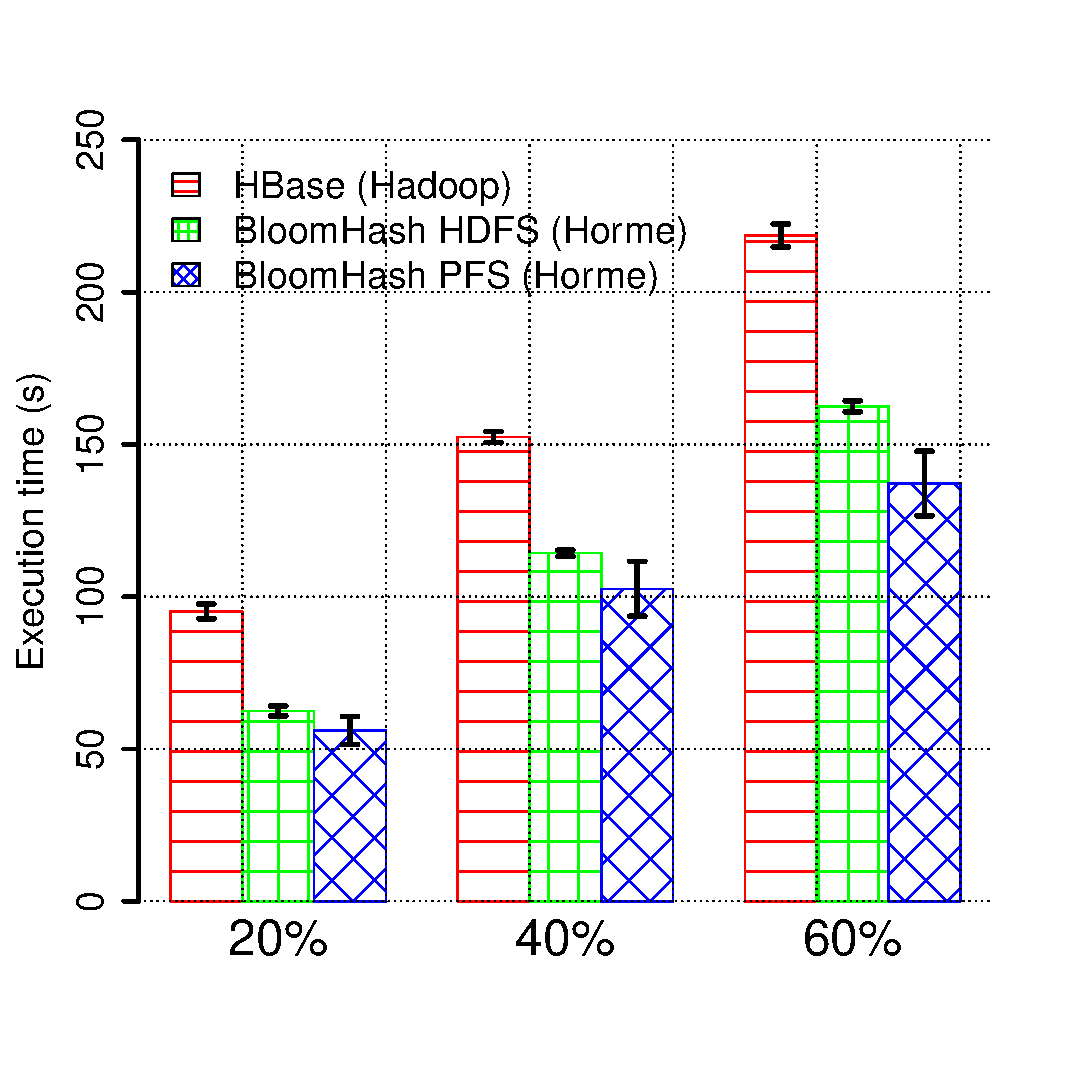
\includegraphics[scale=0.3]{eval-random}
      \centering
      \caption{Query/Random Access}
    \end{figure} 
    \end{column}%
\end{columns}  
\end{frame}

\begin{frame}[c]{Horme vs Vanilla Hadoop}
\begin{figure}[ht!]
      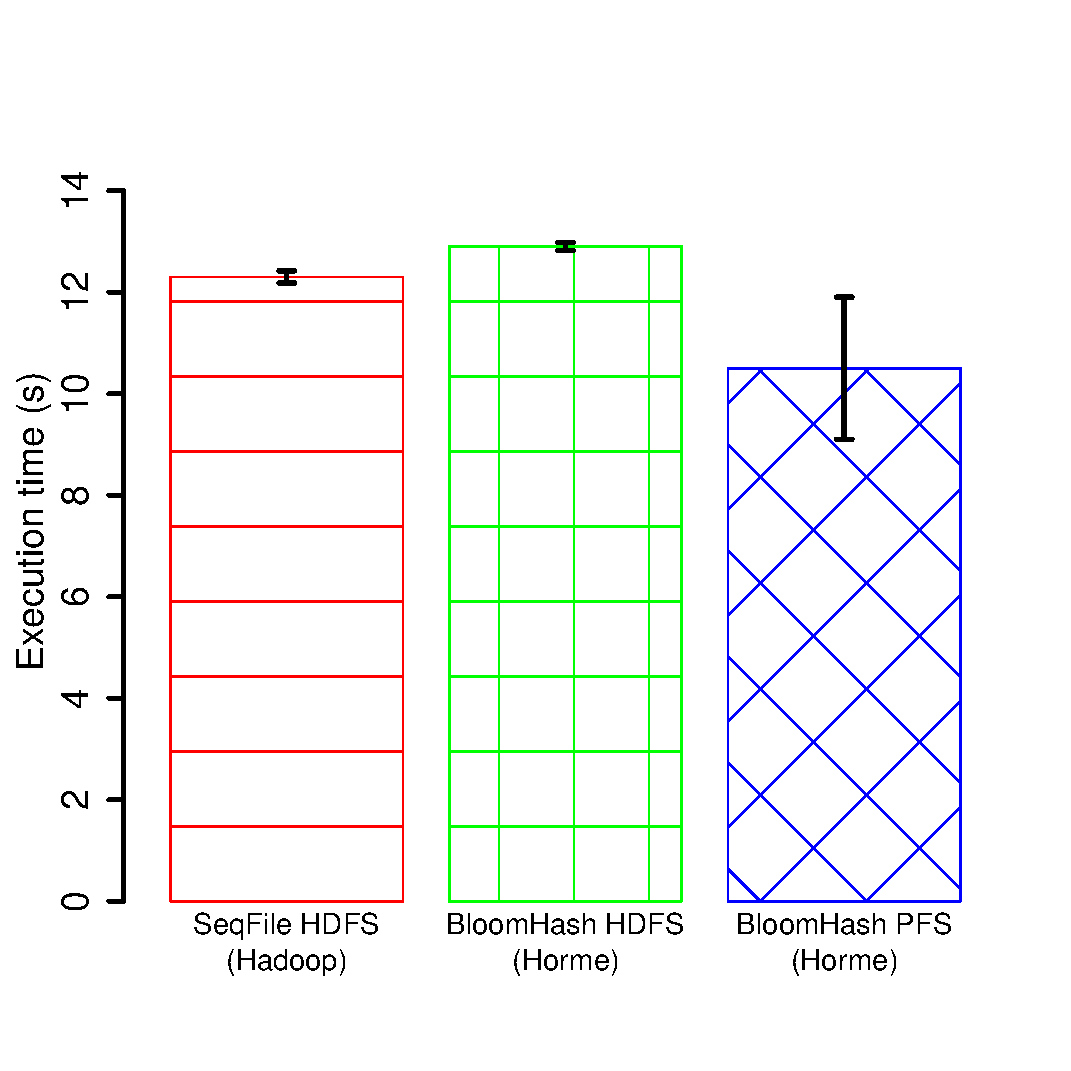
\includegraphics[scale=0.3]{eval-write}
      \centering
      \caption{Write}
    \end{figure}  
\end{frame}

\begin{frame}[c]{Observations}
  \begin{itemize}
    \item Horme’s “Random read from PFS” outperforms Hadoop’s “Random read from HBase” by 41.1%, 32.7%, and 37.3% for 20%, 40% and 60% query setting, respectively. 
    \item It is also superior to “Random read from HDFS” by 10.8%, 10.2% and 15.6% respectively in the three settings.
  \end{itemize}
\end{frame}
\end{document}